\section{Detector calibration}
\label{sec:calibration}	
EASIER detectors  are required to measure faint  and impulsive signal.
A figure  of merit  of the  sensitivity used in  the field  is usually
given by:
\begin{equation}
\rm  F  =  \frac{k_{B}\cdot  T_{sys} }{A_{eff}\cdot  \sqrt{\Delta  \nu
    \Delta t}}
\label{eq:sensitivity}  
\end{equation}
F  represents the  flux  from a  signal  that would  equate the  noise
fluctuation;  $\rm T_{sys}$  is  the noise  system temperature, it is the sum of the thermal noise collected by the antenna and the electronics noise  added mainly by the first amplifier; $k_B$ is  the Boltzmann constant;  the square  root term is the amount of samples  over which this noise is  averaged, in simple case
it is the product of the  bandwidth $\Delta f$ with a time constant of
a low pass filter but in the  case of transient signal, it is meaningful
to use the expected duration of the signal. Finally, $\rm A_{eff}$ is
the effective  area of the antenna  i.e.  the portion  of the incoming
radio flux transformed into electrical power.
\subsection{sensor calibration}
%The   sensor,  the   antenna  and   the  LNB,   will   participate  in
%eq.~\ref{eq:sensitivity}  in   most  of   the  term.
\paragraph{antenna effective area}
The effective area is derived from the knowledge of the antenna gain pattern, i.e. the gain of the antenna as a
function of the direction.
Indeed, the effective area for a particular wavelength $\lambda$, in  a given direction $\theta, \phi $ can be expressed as:
\begin{eqnarray} \label{aeff}
\rm A_{eff} (\theta, \phi) = {{\lambda^2\ G(\theta, \phi)}\over{4 \pi} } 
\end{eqnarray}
The gain pattern can be either measured or simulated. 
 It has been measured for the antenna DMX241 from WS International (Fig.~\ref{fig:wsi-imep}-top),  and for an ATM horn coupled to a LNB Norsat
  in an anechoic chamber at the IMEP (Institut de
Microelectronique Electromagnetique et Photonique) at
Grenoble. The angular dependence of the effective area is illustrated  in Fig.~\ref{fig:wsi-imep}-bottom.
\begin{figure}[ht]
\centering
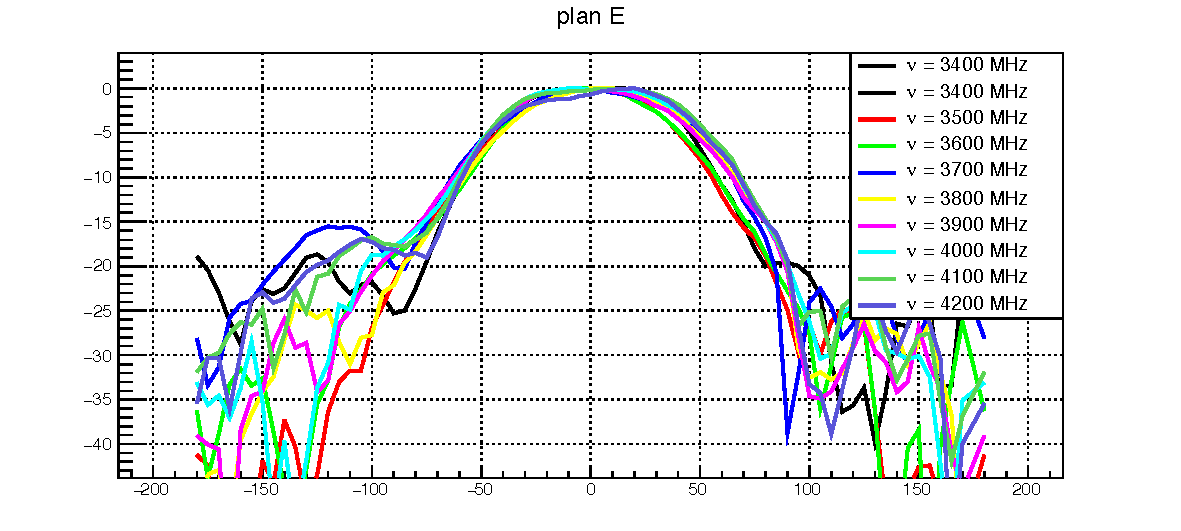
\includegraphics[width=0.49\linewidth]{../plots/C_wsi_g_E.pdf}
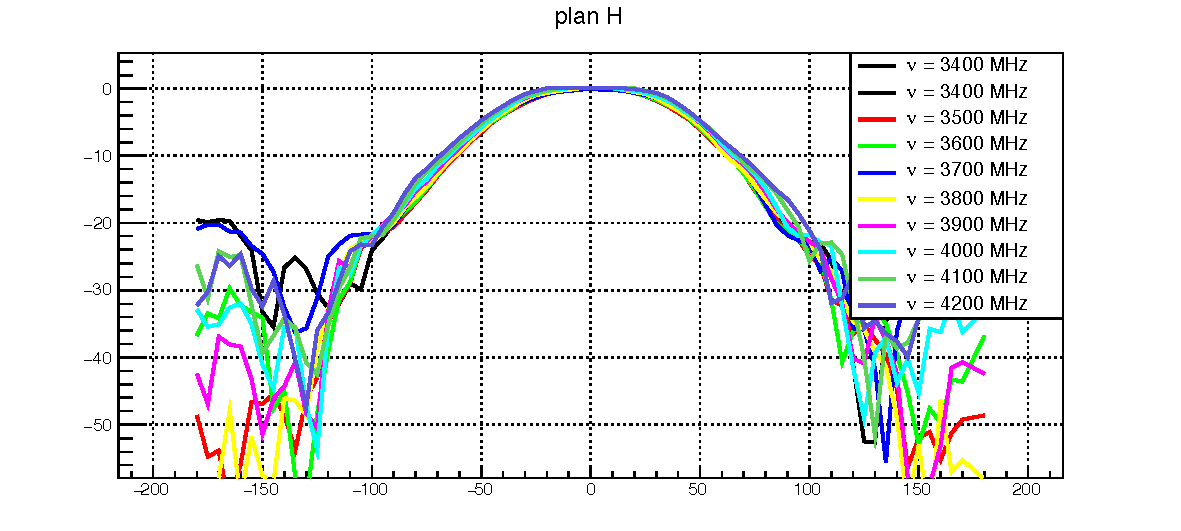
\includegraphics[width=0.49\linewidth]{../plots/C_wsi_g_H.pdf}\\
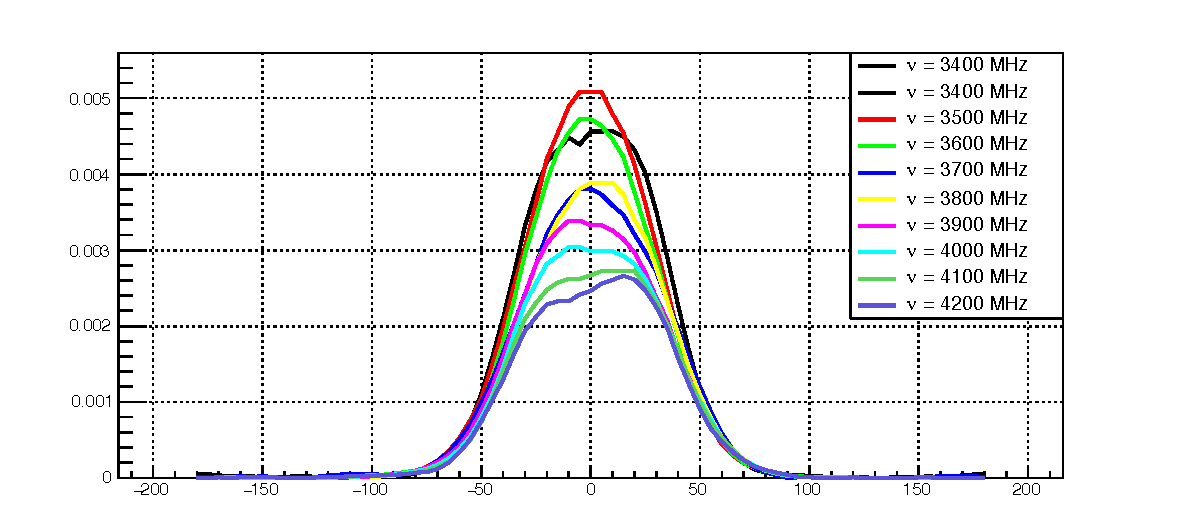
\includegraphics[width=0.55\linewidth]{../plots/C_wsi_A_EH.pdf}\\
\caption{Top: gain measurements in H and E planes- Bottom : corresponding effective area}
\label{fig:wsi-imep}
\end{figure}  
 In addition to these measurements, 
the High Frequency Simulation Software (HFSS) from ANSYS was used to simulate the
patterns of the different tested antenna types, taking into account the setup of the sensors, such as the presence of a radome.
% It  allows modeling the effect of the ground, water tank and all the surroundings on the antenna pattern.
Two different pyramidal horns (ATM and A-INFO) with 15~dB gain were simulated using HFSS~\cite{HFSS} to retrieve their gain patterns with the same free space conditions, at 3.8 GHz (Fig.~\ref{fig:A-INFO_radome}). Gain and beamwidth values from the simulation results are found to be compatible with the spreadsheets.
% as shown  in Table ~\ref{tab:pyramidal-horns}. 
A compromise between the expected performances and the cost led to the selection of seven A-INFO type horns.

\begin{figure}[ht]
\centering
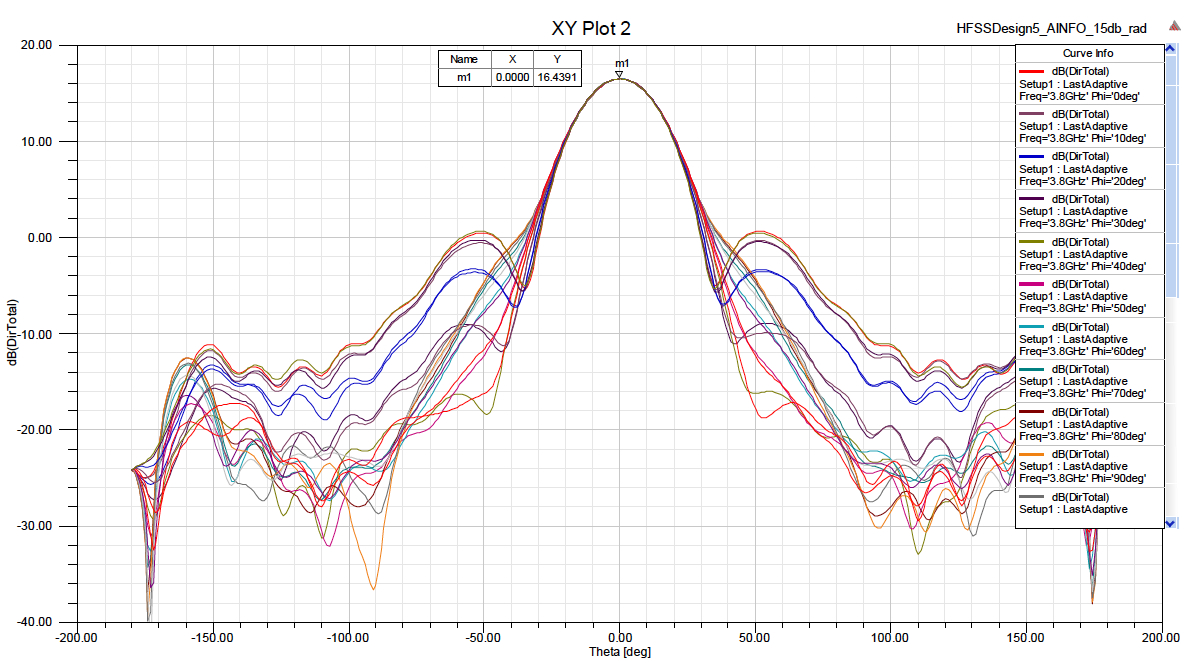
\includegraphics[width=0.5\textwidth]{../plots/AINFO_15dB_radome_pattern_HFSS.jpg}
\caption{\small{A-Info diagram with radome}}
\label{fig:A-INFO_radome}
\end{figure}  
A radome consisting of a plexiglas slab had to be fixed on the horn aperture to shield the antenna against UV, humidity. The attenuation effect of this plexiglas slab (2~mm thick, protected against UV) was evaluated using HFSS : the loss $L$ is found to be 0.17~dB. The power loss measured in the half spherical radome used for the standard EASIER61 antennas gives 0.5 dB ($\sim$31 K), more important than found for these new antennas.


%\paragraph{antenna temperature}
%The system temperature makes use of the effective area...
\subsubsection{system noise temperature}
%The noise in the EASIER and GIGADuck radio system is the sum of the antenna temperature estimated according the Eq~\eqref{tant} and the electronics noise  temperature which main contributor is the first amplifier.
%arise from on one side the thermal noise of the surrounding material collected by the antenna lobe, the antenna temperature $\rm T_{ant}$ and on the other side the electronics noise $\rm T_{elec}$.  It is  related to  the system power $\rm P_{sys}$ through:
%\begin{equation}
%  \rm  P_{sys}  =  k_{B} T_{sys}  G  \Delta  \nu  = k_{B}  (T_{ant}  +
%  T_{elec}) G \Delta \nu
%\end{equation}
%with G the electronics gain and $\rm \Delta  \nu$ the bandwidth.  The system temperature of a device is measured by comparing the output of the device when two different sources of noise are applied to its input. This method permits to cancel out the gain term in the calibration equation. A common method is to make use of an astronomical source with an known flux as a calibration source. This method is suitable when the flux is intense enough to be observed in the device. We used the sun as a calibration source to calibrate the GIGADuck detectors, see section~\ref{sec:gdtsys}. For EASIER detector and their smaller gain antenna, this method couldn't be used. Instead we setup a simple experiment consisting of the comparison of the signal when the antenna look down to the ground and when it looks up in the sky.
\paragraph{EASIER61}
The method implemented to measure the electronics noise temperature of the EASIER61 detectors relies on the so called Y-factor method. It extracts the noise temperature of a device, here the EASIER61 electronics, with the measurement of two different input noise powers. In the case of EASIER61 we simply pointed the antenna toward the ground and then toward the sky so that the electronics is subjected to two different antenna temperature. Then the temperature is found with the following equation:
\begin{equation}
	\rm	T_{elec} = \frac{T_{hot} - YT_{cold}}{Y-1} \ where \ Y = \frac{P_{hot}}{P_{cold}}
\end{equation}
where $\rm T_{hot}$ ( $\rm T_{cold}$ ) is the antenna temperature when the antenna points toward the ground (the sky) and $\rm P_{hot}$ ($\rm P_{cold}$) are the corresponding powers. The antenna temperatures are computed according:
\begin{equation}
\rm  T_{ant} = \rm \int_{\theta =  0}^{\theta = \pi}\int_{\phi = 0}^{\phi =
    2\pi} T_{B}(\theta) G(\theta,\phi) \sin(\theta) d\theta d\phi
\label{eq:tant}
\end{equation}
with $\rm T_{B}(\theta)$ the brightness temperature, around \unit[4]{K} for the sky at the zenith and \unit[270]{K} for the ground. Antenna temperatures if  $\rm T_{hot} = \unit[260]{K}$ and $\rm T_{cold} = \unit[6]{K}$ are obtain. \\ The measurement took place in the pampa at the detector's site. The setup comprises the main component of the installed detectors namely the LNBf, the radome and the power detector Minicircuit ZX47-50. The antenna was oriented consecutively up and down and the voltage of the power detector was recorded with a portable oscilloscope. The voltage difference between the two measurement is related to a difference of power according the calibration curve  of the power detector (see section~\ref{sec:calibration}). For the two types of LNBf used in EASIER61, we found system noise temperatures of $\rm T^{GSI}_{elec} =  \unit[114]{K} \pm 10$ and $\rm  T^{DMX}_{elec}  =  \unit[97]{K}   \pm  9$. The errors include an uncertainty on the calibration factor in Eq.~\eqref{eq:delvdelp} of 1mV/dB and a spread of the ground brightness temperature of $\rm \pm \unit[10]{K}$ due to the poorly known physical temperature and emissivity.


%Because the measurement of the gain with a high precision is hard to achieve, the main method to retrieve the system
%temperature  is to  combine two  measurements with  a  different input
%noise power -  or the equivalent temperature - to  cancel out the gain
%term.  The  system noise temperature  of EASIER and GIGAS's  LNBf were
%measured by  the CROME collaboration  comparing the output  power when
%the  antenna collects noise  from surrounding  material first  at room
%temperature       and        then       at       liquid       nitrogen
%temperature~\cite{bib:gapnoteCROME}.   The electronics  temperature of
%the GI 301 was  found to be very variable from 40  to 180K, the one of
%the WS  International stable  at 25K and  the Norsat at  23.5K.  MIDAS
%experiment  uses  also  the  LNBf  WSI DMX241  and  measured  a  noise
%temperature  of  25K~\cite{bib:midas}.   We  have  also  measured  the
%electronics noise temperature of  the WSI DMX241 comparing the spectra
%measured at room temperature in  laboratory when the antenna is facing
%an absorber ($\rm T_{room} = \unit[300]{K}$) with the measurement when
%the  antenna faces  the  sky ($T_{sky}  = \unit[7]{K}$).   \textit{The
%  results   we  obtain  for   amounts  to   around  $\rm   T_{elec}  =
%  \unit[40]{K}$.     The   difference   with    previously   mentioned
%  measurements can  be explained  by the radome  protection.}
\paragraph{GIGADuck}
For the GIGADuck antennas, since their gain is larger, the sun passage is observed in the monitoring data and can be used as a calibration source.  The increase  of power induced upon the passage of the sun in the antenna field of view reads:
\begin{equation}
  \rm       \unit[\Delta      P]{[dBm]}       =       10      log_{10}
  (\frac{P_{sys} + P_{sun}(\theta_{sun},\phi_{sun})  }{P_{sys}} )  = 10
  log_{10}     (    1     +     \frac{    \frac{1}{2}F_{sun}     \cdot
    A_{eff}(\theta_{sun},\phi_{sun}) } {T_{sys}} )
  \label{eq:deltaP}
\end{equation}
where    $\rm   F_{sun}$    is    the   total    solar   flux which is measured by dedicated solar observatory like~\cite{sundata} or~\cite{nobeyama},    $\rm A_{eff}(\theta_{sun},\phi_{sun}) $ is the antenna effective area for the given position of the sun in  the sky and the factor $\rm \frac{1}{2}$ is  the polarization factor.  This measurement can be performed only when the sun is  in the field  of view of  the antenna. As  it is shown  in the
Fig.~\ref{fig:sunsim} (left), the sun  is not visible by any antenna of the  GIGADuck array  during austral winter  but will cross  the field of view of five of them during summer.\\ We  retrieve the absolute value of  the daily average sun    flux   at   \unit[2.8]{GHz}    measured at the Dominion Radio Astrophysical Observatory and publicly released at~\cite{sundata}.  The  flux at the  center frequency of  the C-band, \unit[3.8]{GHz},   is  obtained   by   using  parameterization   found in~\cite{sunparam, sunparam2}. 
\begin{figure}[!ht]
 \centering
 \hspace*{-3ex}
 \subfigure{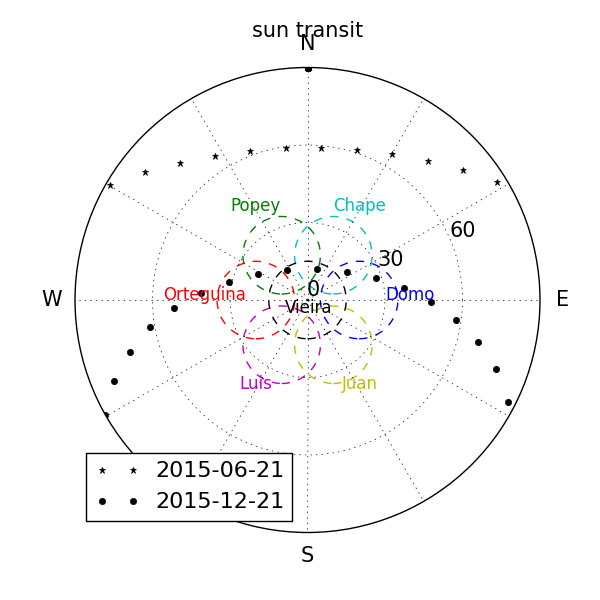
\includegraphics[width=0.39\linewidth]{sunpolar.png}}
 \subfigure{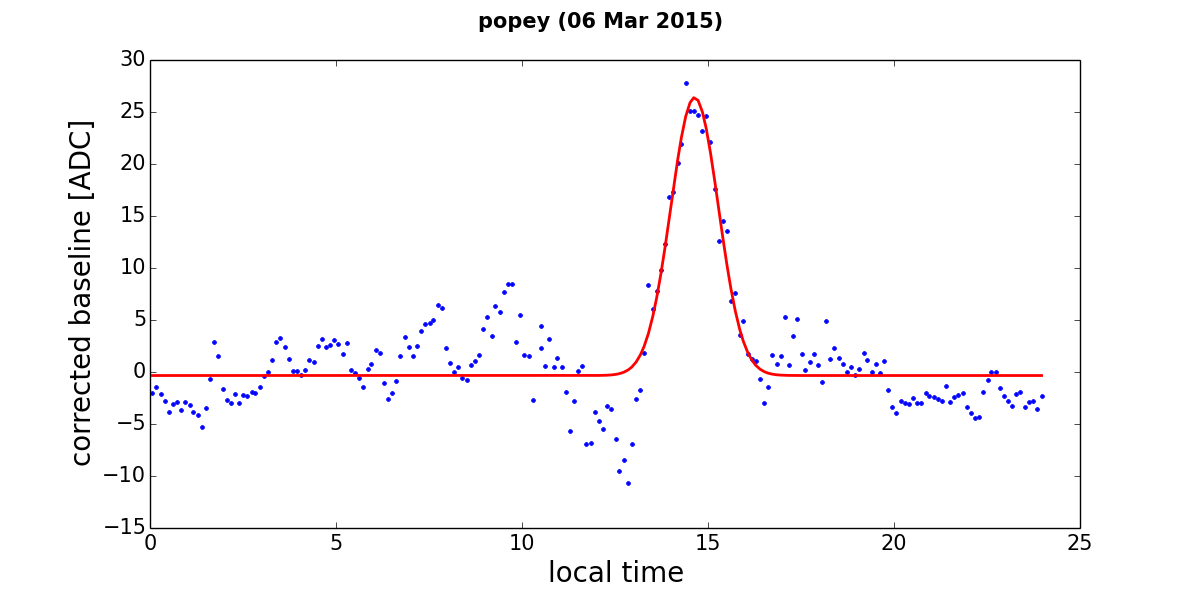
\includegraphics[width=0.6\linewidth]{fitexample.png}}
%% \subfigure{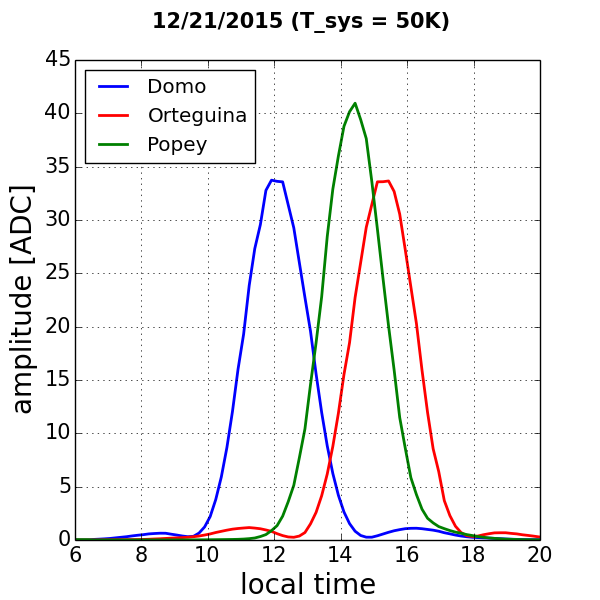
\includegraphics[width=0.49\linewidth]{sunexpected.png}}
 \caption{Left: Sun transit for the two solstices. The colored circles
   represent  the field  of  view of  the  GIGADuck antennas.   Right:
   Example  of the  baseline during  one  day. In  blue is  the
   orignal baseline when the mean is subtracted, in green after it was
   corrected from temperature dependence and  in red is a gaussian fit
   of to extract the signal from the sun.}
%%    Simulated  baseline  increase for  three  antennas  during the  sun
%%    passage.}
 \label{fig:sunsim}
\end{figure}
Since GIGADuck data are  part of  the SD  data stream  including the monitoring system, the radio  baseline is recorded every \unit[400]{s} with other  information such as  the outside temperature. The sun signal is extracted from these data with the following method.  First the rainy periods are removed, since rain and  high humidity  affect the radio  baseline in a non trivial way. Then this data set is used to correct for a linear  dependence of the system's gain with the outside temperature (the time when the sun is expected is removed for this parameterization). The final step consist in fitting the bump induced by the sun flux with a Gaussian function. The maximum of the fitted function is then converted in power difference according Eq.~\eqref{eq:eqcalibration} and the system noise temperature is retrieved with Eq.~\eqref{eq:deltaP}.\\ This method was applied for four antennas and the results for each day for two of them are shown in the Fig.~\ref{fig:GDtempres}. Some measurements show a large error bar due to the uncertainty on the value of the maximum of the baseline that particular day. The obtained temperature are \unit[39, 45, 59 and 70]{K}. The system noise temperature of the three other detectors are taken as the maximum measured to remain conservative.

\begin{figure}[!ht]
 \centering
 \hspace*{-3ex}
 \subfigure{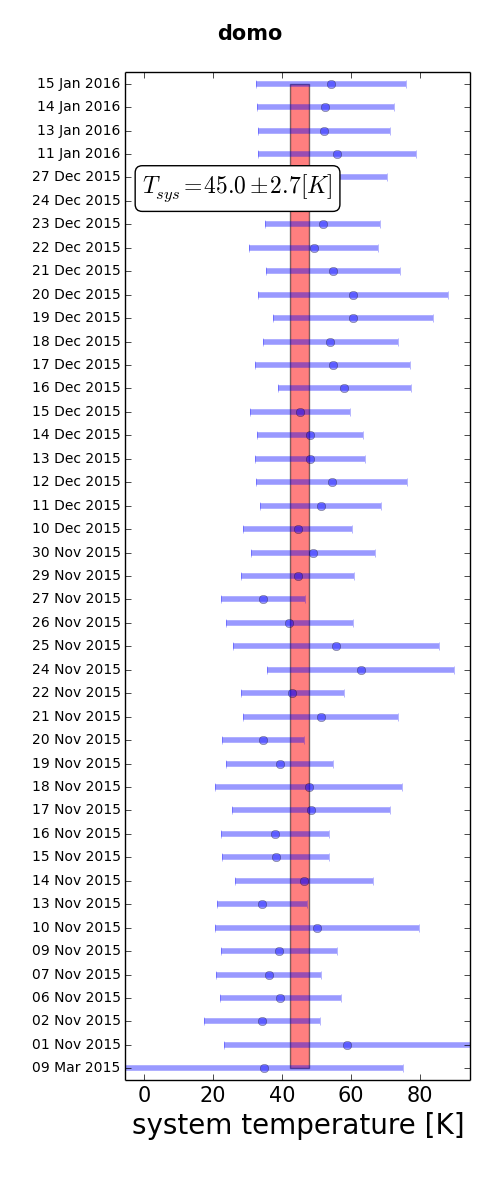
\includegraphics[width=0.25\linewidth]{domosystemp.png}}
  \subfigure{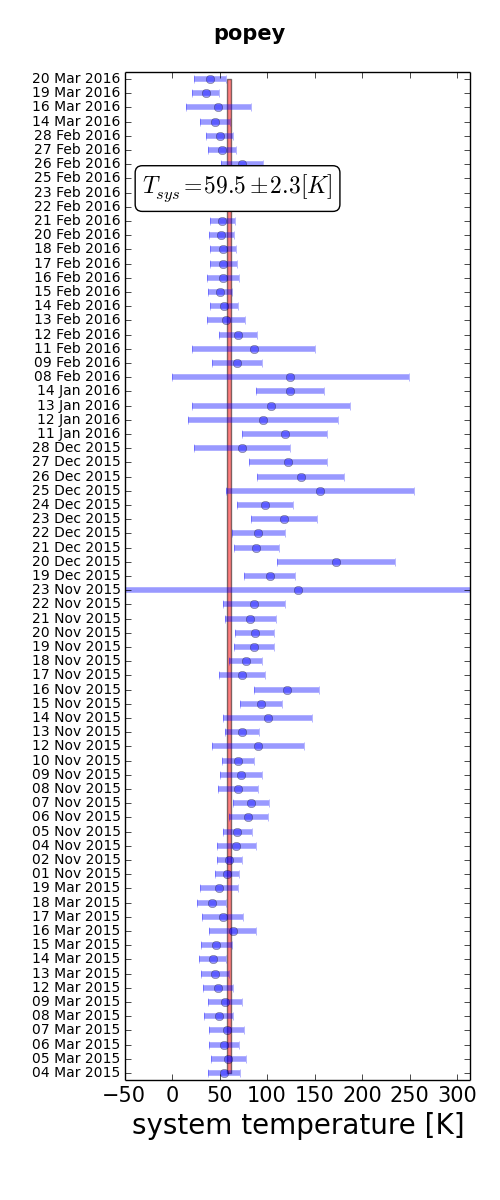
\includegraphics[width=0.25\linewidth]{popeysystemp.png}}
  \caption{Temperature measured for two GIGADuck detectors with the sun signal.}
 \label{fig:GDtempres}
\end{figure}


\paragraph{sensor bandwidth}
The absolute gain  of the RF part which includes the amplifier the bias tee, the cables etc, does  not  enter  directly in  the  detector's sensitivity,     but    the     frequency    bandwidth     does    (cf eq.~\ref{eq:sensitivity}).  The  normalized gain  of the LNB  used for EASIER61 (GI301, DMX241) and GIGADuck (Norsat 8115) are represented in the  Fig.~\ref{fig:normalizedgain}  and  the  effective  bandwidth  is computed according:
\begin{equation}
  \rm \Delta \nu = \frac{1}{G_{max}} \int G(f) \cdot df
\end{equation}
We  obtain effective bandwidths  of \unit[437  $\rm \pm$  30]{MHz} and
\unit[445 $\rm \pm$ 56]{MHz} for the GI301 and the DMX241 respectively
and \unit[750]{MHz} for the Norsat.
\begin{figure}[!ht]
  \centering
  \hspace*{-3ex}
 \subfigure{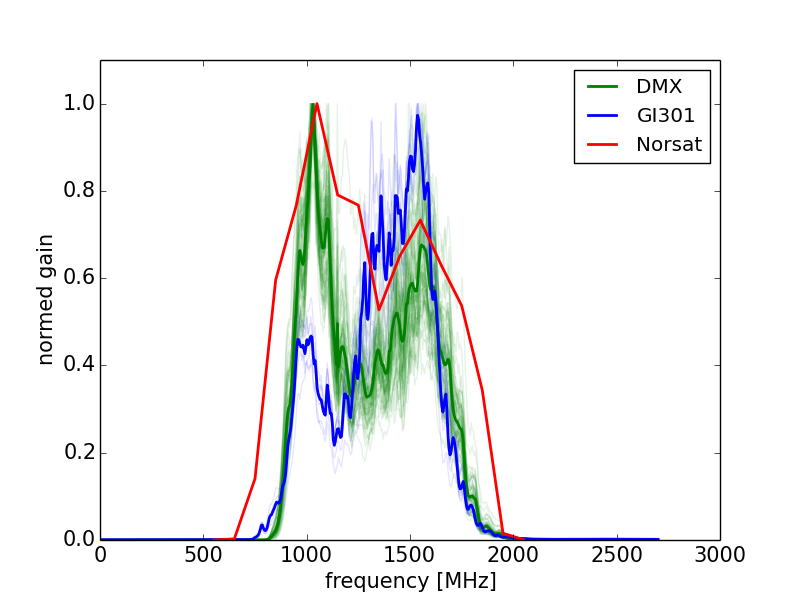
\includegraphics[width=0.49\linewidth]{spectra3.png}}
  \caption{Normalized  gain  of the  three  mentioned  LNBf after  the
    frequency downconversion.  The thick blue and green  lines are the
    average over several detectors. Only one measurement was performed
    with the Norsat LNBf (in red). }
  \label{fig:normalizedgain}
\end{figure}


\subsection{Adaptation electronics calibration}
\label{sec:elec}
\subsubsection{Specification}
The adaptation electronics is composed of the power detector, the adaptation board and ends the analog to digital converter of the Auger SD.  The power detector is an Analog Device AD8318 (in the encapsuled version Minicircuits ZX47-50), it is  a logarithmic  amplifier with a  wide bandwith and  large power
dynamic  range.  For the first seven detectors its output  voltage  was  filtered  with  an  output capacitor  but this capacitor is removed for  the  following version   EASIER61  and  GIGADuck.  The power detector output voltage $\rm V_{pd}$ was calibrated in laboratory using a noise waveform at various power $P_{in}$ as input:
\begin{equation}
  \rm  V_{pd} [V] =  -0.0234\cdot P_{in} [dBm] + offset
\label{eq:eqpd}
\end{equation}
 The  power detector  voltage is  then amplified  by a  factor  4.2 to
 obtain  a final  power dynamics  of \unit[20]{dB}  over the  1024 ADC
 counts of the  SD acquisition. The overall conversion  from the input
 power to the ADC is:
\begin{equation}
  \rm ADC = 50.2\cdot P [dBm] + offset
\label{eq:eqcalibration}
\end{equation}
An offset was designed to be adjustable to make up for the differences of the detectors gain.

\subsubsection{Time response and electronics simulation}
In  the  following  paragraphs  we  study the  time  response  of  the
adaptation  electronics. 
\paragraph{power detector}
To understand the power detector response to impulsive signals, we set  a detection chain in laboratory composed  of a LNBf  followed by a  power detector. A fast oscilloscope is  used to record simultaneously the  LNBf and power
detector's  output. We  used the  spark  of an  electronic lighter  to
produce a short and broadband  signal and emulate  the signal from an  air shower. An example of these signal is shown in the Fig.~\ref{fig:powerdetsim}. We  find that the power detector output is well reproduced when one perform  a convolution of the input signal in dBm (logarithmic unit) and an exponential function with a decay constant $\rm \tau$:
\begin{equation}
  \rm V_{PD}(t) = k_{1}\cdot \int_{t>0}P_{dBm}(u)exp(\frac{t-u}{\tau})du + k_{2}
  \label{eq:convolution}
\end{equation}
The factor    $\rm   k_{1}$  is fixed to   the   conversion    factor   of   the
equation~\ref{eq:eqpd} and $\rm   k_{2}$ is an offset. We simulate fake waveforms from measured RF signal with various decay times  $\rm \tau$. The best $\rm \tau$ is found by minimizing the distance $\rm d = \Sigma (V_{measured} - V_{simulated})^2$ between simulated and measured power detector waveforms.  We found $\rm \tau_{capa}  = \unit[41.5]{ns}$ when an  output capacitor follows the power detector and $\rm \tau_{nocapa} = \unit[6.3]{ns}$ without. 
\begin{figure}[!ht]
 \centering
 \hspace*{-3ex}
 \subfigure{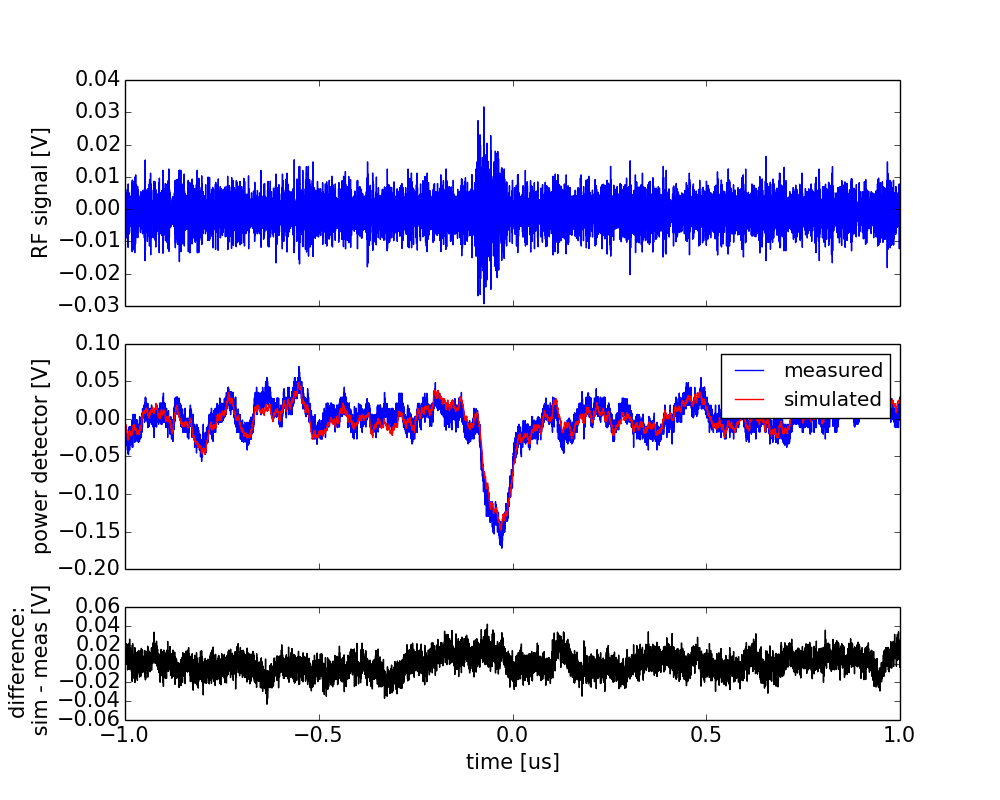
\includegraphics[width=0.7\linewidth]{capa_method3.png}}
 \caption{Example  of RF  and power  detector waveforms.  The measured
   waveforms are in blue and the simulated one in red. The lower panel
   show the difference.}
 \label{fig:powerdetsim}
\end{figure}
\paragraph{Adaptation board}
To measure the response of  the adaptation board, we add it to the calibration setup described in the previous paragraph.  We  recorded simultaneously the  input of the  board and  its  output. We  find the  board's response  by measuring the its transfer function in the frequency domain:
\begin{equation}
  \rm \tilde{H}(f) = \frac{\tilde{V}_{out}(f)}{\tilde{V}_{in}(f)}
\end{equation}
The  gain and the phase of the board is  represented  in  the  Fig.~\ref{fig:board}. \\The last part of  the chain, the Auger front  end is simulated with  a low pass filter with $\rm f_{cut} = \unit[20]{MHz}$ and by sampling in time and amplitude.
\begin{figure}[!ht]
 \centering
 \hspace*{-3ex}
 \subfigure{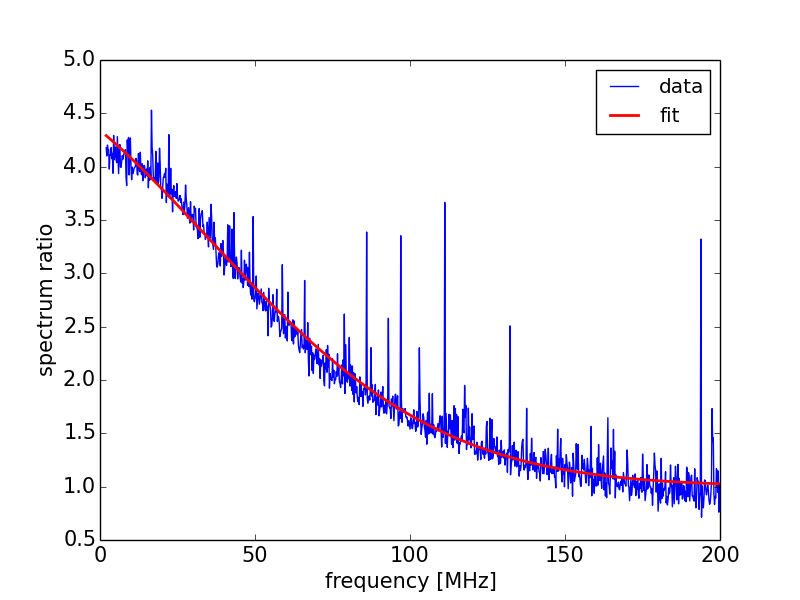
\includegraphics[width=0.49\linewidth]{fitspecboard2.png}}
 \subfigure{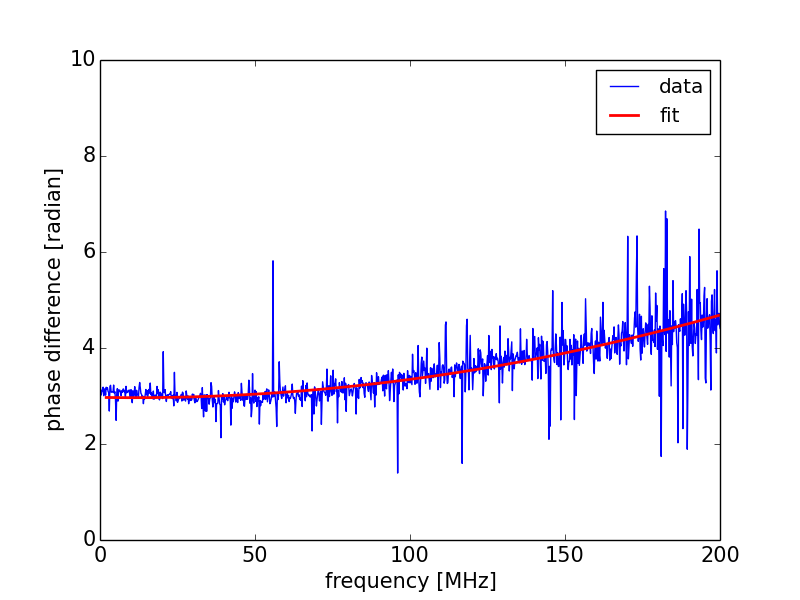
\includegraphics[width=0.49\linewidth]{fitphaseboard.png}}
 \caption{Measurement and fit of the gain and phase of the adaptation board.}
 \label{fig:board}
\end{figure}

\paragraph{validation with data}
In order to  validate the calibration and simulation,  we produced some mock data   
and compare them with the  actual radio waveform  we record in  the Auger data.   An RF waveform   is  generated   from   the  spectra   represented  in   the Fig.~\ref{fig:normalizedgain}   by  inverse  FFT.    The  adaptation electronics simulation  is then applied to  it in order  to produce an trace    in   ADC    count.     The Fig.~\ref{fig:distcomparison} the distribution  of the noise for the
data (in grey)  and the simulation (in red).  The comparison are shown
for the three setups.
\begin{figure}[!ht]
 \centering
 \hspace*{-3ex}
 \subfigure{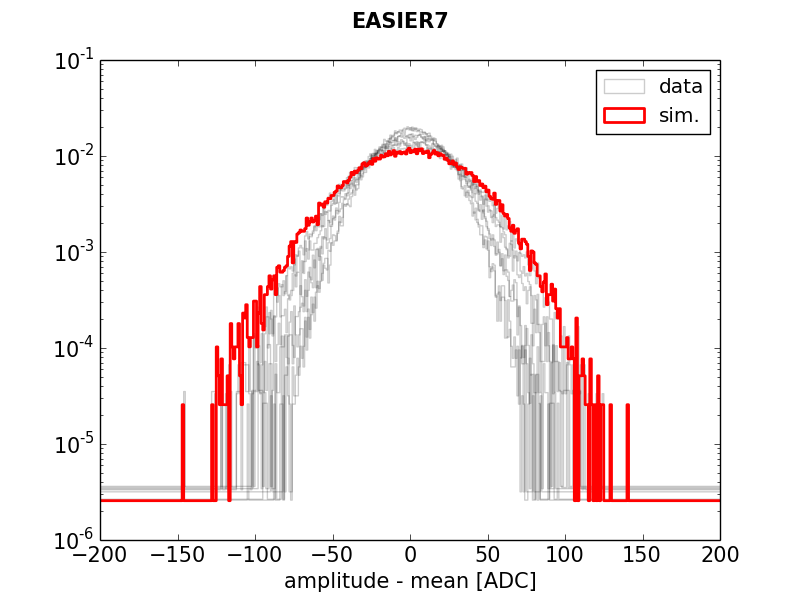
\includegraphics[width=0.32\linewidth]{m3_distdatasimEA7.png}}
 \subfigure{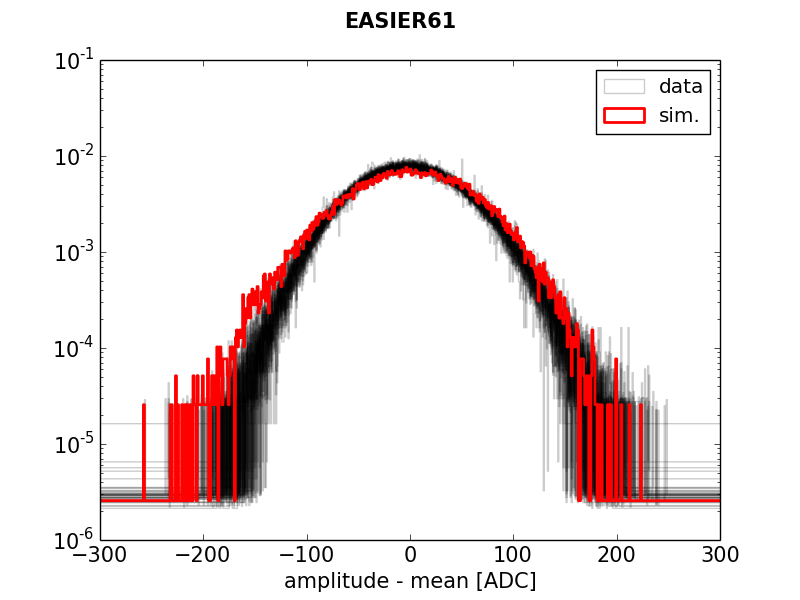
\includegraphics[width=0.32\linewidth]{m3_distdatasimEA61.png}}
 \subfigure{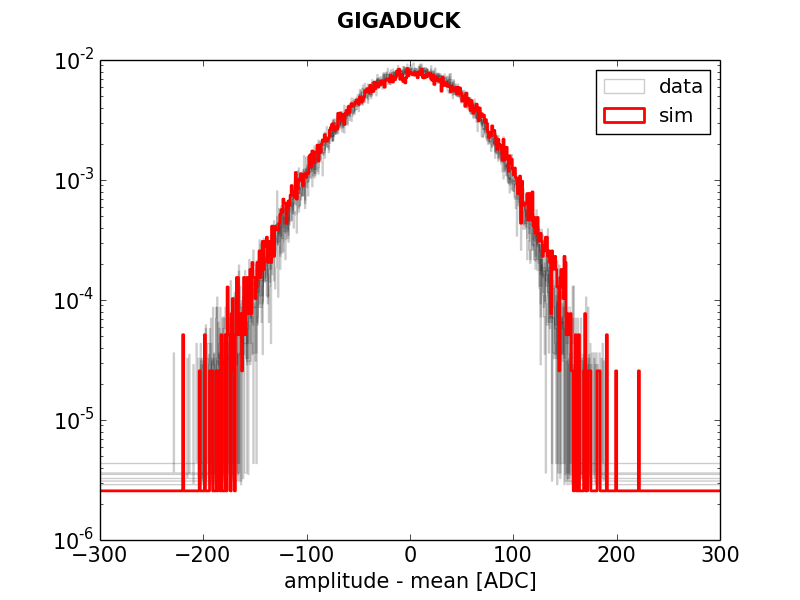
\includegraphics[width=0.32\linewidth]{m3_distdatasimGD.png}}
 \caption{Distribution of the waveform value for simulated and measured data for the EASIER61 setups (left and middle) and for the GIGADuck setup (right)}
 \label{fig:distcomparison}
\end{figure}
If the simulations agree very well for EASIER61 and GIGADuck, it tends
to overestimate the noise fluctuation for the first setup. However the
measured and simulated standard  deviation of the distributions differ
 at maximum by 15 ADC counts which represent \unit[0.3]{dB} or 7\%.

